\documentclass[10pt,a4paper, margin=1in]{article}
\usepackage[utf8]{inputenc}

\usepackage{fullpage}
\usepackage{amsfonts, amsmath, pifont}
\usepackage{amsthm}
\usepackage{graphicx}
\usepackage{tikz}
\usepackage{float}
\usepackage{tkz-euclide}
\usepackage{pgfplots}
\pgfplotsset{compat=1.13}
\begin{filecontents}{q3.dat}
 n   xn
 -11  6
 -10  0
 -9   5
 -8   0  
 -7   -4
 -6   0
 -5   0 
 -4   3
 -3   0
 -2   -2
 -1   0
 0   1
 1  1
 2  0
 3  0
 4  -4
 5  5
 6  6
\end{filecontents}

\usepackage{geometry}
 \geometry{
 a4paper,
 total={210mm,297mm},
 left=10mm,
 right=10mm,
 top=10mm,
 bottom=10mm,
 }
 % Write both of your names here. Fill exxxxxxx with your ceng mail address.
 \author{
  Civelek, Seda\\
  \texttt{e2237147@ceng.metu.edu.tr}
  \and
  Shikhaliyev, Emil\\
  \texttt{e2280386@ceng.metu.edu.tr}
}
\title{CENG 384 - Signals and Systems for Computer Engineers \\
Spring 2020 \\
Written Assignment 1}
\begin{document}
\maketitle



\noindent\rule{19cm}{1.2pt}

\begin{enumerate}

\item 
    \begin{enumerate}
    % Write your solutions in the following items.
    \item %write the solution of q1a
  
   
    $z+3\overline{z}=j-1$ \\
    $x+jy+3(x-jy)=j-1$ \\
    $4x-2jy=j-1$ \\
    $x=\dfrac{-1}{4},$ $y=\dfrac{-1}{2}$ \\
    $|z|^2 = x^2 + y^2$ \\
    $|z|^2 = \dfrac{1}{16}+\dfrac{1}{4}=\dfrac{5}{16}$ \\
    
	
	\begin{figure}[!htbp]
    	\begin{center}
        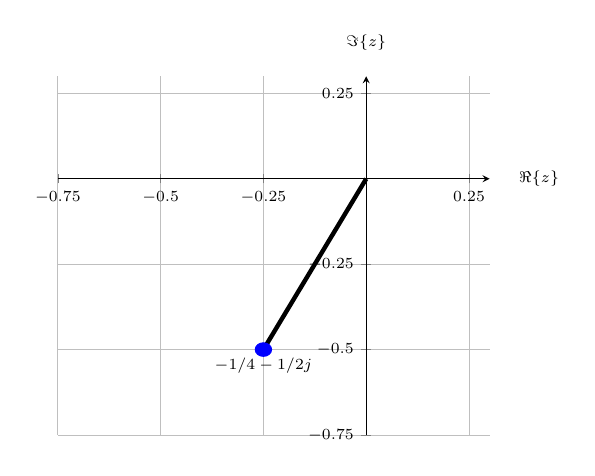
\begin{tikzpicture}[scale=0.8]
        \begin{scope}[thick,font=\scriptsize]
           \begin{axis}[
          axis lines=middle,
          xlabel={$\Re\{z\}$},
          ylabel={$\Im\{z\}$},
          xtick={-0.75,-0.5,-0.25,0,0.25},
          ytick={-0.75,-0.5,-0.25,0,0.25},
          ymin=-0.75, ymax=0.3,
          xmin=-0.75, xmax=0.3,
          every axis x label/.style={at={(ticklabel* cs:1.05)}, anchor=west,},
          every axis y label/.style={at={(ticklabel* cs:1.05)}, anchor=south,},
          grid,
        ]
           \path[draw,line width=2pt] (0,0) -- (-0.25,-0.5);
           \draw [color=blue, fill=blue] (-0.25,-0.5) circle(0.02);
           \node [color=black] at (-0.25,-0.5) [below]{$ -1/4-1/2j$};
           \end{axis}
           \end{scope}
        \end{tikzpicture}
        \caption{$z$ on the complex plane.}
        \end{center}
    \end{figure}
    
    \item %write the solution of q1b 
	
	$z=a+jb$\\
	$a=r\cos\theta,$ $ b=r \sin\theta$\\
	$z=r\cos\theta + jr \sin\theta$\\
	$z^2=r^2(\cos^2\theta-\sin^2\theta)+j2r^2\cos\theta \sin\theta$\\
	$\cos^2\theta-\sin^2\theta =0$\\
	$\theta=\pi/4$\\
	$r^2\sin2\theta = 25$ \\ $r=5$\\
	$z=5e^{j(\pi/4+\pi k)}$\\
	$z_0=5e^{j\frac{\pi}{4}}$ for k=0\\
	$z_1=5e^{j\frac{5\pi}{4}}$ for k=1\\
    
    \item %write the solution of q1c
    $z = \dfrac{(1+j)(1-\sqrt{3}j)}{1-j} = \dfrac{(1+j)(1+j)(1-\sqrt{3}j)}{(1-j)(1+j)}$ multiplying both numerator and denominator with $(1+j)$\\
    $z=\dfrac{2j \cdot (1-\sqrt{3}j)}{2}$\\
    $z=\sqrt{3}+j$\\
    $r=\sqrt{3+1}=2$\\
    $\theta = \tan^{-1}(\dfrac{1}{\sqrt{3}})=\pi/6$\\
	    
    
    \item %write the solution of q1d
    
    $j=e^{j\pi/2}$\\
    $z=je^{-j\pi/2}=e^{j\pi/2}e^{-j\pi/2}=e^0=1$
    \end{enumerate}
\newpage
    \item %write the solution of q2
    \textbf{}\\
	\begin{figure}[]
    	\begin{center}
        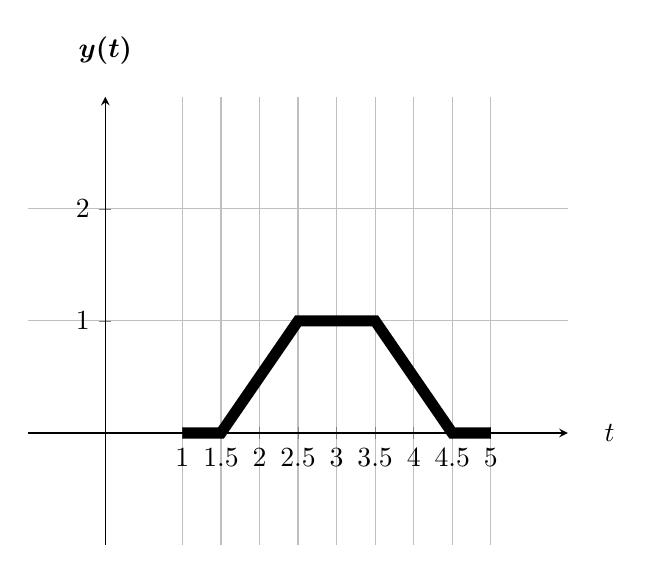
\begin{tikzpicture}[scale=1.0]
           \begin{axis}[
          axis lines=middle,
          xlabel={$t$},
          ylabel={$\boldsymbol{y(t)}$},
          xtick={0, 1,1.5, 2,2.5, 3,3.5,4,4.5, ..., 5},
          ytick={0, 1, 2},
          ymin=-1, ymax=3,
          xmin=-1, xmax=6,
          every axis x label/.style={at={(ticklabel* cs:1.05)}, anchor=west,},
          every axis y label/.style={at={(ticklabel* cs:1.05)}, anchor=south,},
          grid,
        ]
           \path[draw,line width=4pt] (1,0) -- (1.5,0) -- (2.5,1) -- (3.5,1) -- (4.5,0) -- (5,0);
           \end{axis}
        \end{tikzpicture}
        \caption{$t$ vs. $y(t)$.}
        \end{center}
    \end{figure}
    
\item      
    \begin{enumerate}
    \item %write the solution of q3a
     \textbf{}\\
    \begin{figure} [h!]
    \centering
    \begin{tikzpicture}[scale=2] 
      \begin{axis}[
          axis lines=middle,
          xlabel={$n$},
          ylabel={$\boldsymbol{x[-n]+x[2n-1]}$},
          xtick={ -11,..., 0,  ..., 6},
          ytick={-4, -3, -2, -1, ..., 6},
          ymin=-5, ymax=7,
          xmin=-12, xmax=7,
          every axis x label/.style={at={(ticklabel* cs:1.05)}, anchor=west,},
          every axis y label/.style={at={(ticklabel* cs:1.05)}, anchor=south,},
          grid,
        ]
        \addplot [ycomb, black, thick, mark=*] table [x={n}, y={xn}] {q3.dat};
      \end{axis}
    \end{tikzpicture}
    \caption{$n$ vs. $x[-n]+x[2n-1]$.}
    \label{fig:q3}
\end{figure}
    
    
    \item %write the solution of q3b
    
    $x[-n]+x[2n-1] = 6\delta[n+11]+5\delta[n+9]-4\delta[n+7]+3\delta[n+4]-2\delta[n+2]+\delta[n]+\delta[n-1]-4\delta[n-4]+5\delta[n-5]+6\delta[n-6]$ \\ \\ \\ \\ \\ \\
    \end{enumerate}

\item 
    \begin{enumerate}
    \item %write the solution of q4a
    \begin{enumerate}
        \item 
        $7\sin[\dfrac{5\pi}{8}n-\dfrac{2\pi}{3}]=7\sin[\dfrac{5\pi}{8}(n-\dfrac{16}{15})]$\\
    \\
    $N_0 = \dfrac{2\pi}{\Omega_0}k$\\ \\
    $N_0 = \dfrac{2\pi \cdot 8}{5\pi}k=16k$\\ \\
    $k=5,$ $N_0=16$\\
        \item
        $2\cos[\dfrac{2\pi}{3}n]$\\ \\
        $N_0=\dfrac{2\pi \cdot 3}{2\pi}k=3k$\\ \\
        $k=1,$ $N_0=3$\\
        
    \end{enumerate}
    The fundamental period of the signal is the least common magnitude of the component of the compound signal.\\
    $LCM(16,3)=48$. So the period of $x[n]$ is 48.
    
    \item %write the solution of q4b
    
    $x[n]=3\cos[5(n-\dfrac{3\pi}{20})]$\\
    $N_0=\dfrac{2\pi}{\Omega_0}k$ \\ \\ $\Omega_0=5$\\ \\ 
    $N_0=\dfrac{2\pi}{5}k$\\
    This signal $x[n]$ is not periodic because, there is no integer k value that makes this signal periodic. 
    
    \item %write the solution of q4c
    
    $x(t) = 4\sin(5\pi t-\dfrac{3\pi}{5})=4\sin(5\pi(t-\dfrac{3}{25}))$\\
    $\omega_0=5\pi$\\  
    $T_0=\dfrac{2\pi}{\omega_0}$ \\ \\  $T_0=\dfrac{2\pi}{5\pi}=\dfrac{2}{5}$\\ \\
    
    \item %write the solution of q4d
    
    $j=e^{j\dfrac{\pi}{2}}$\\
    
    $x(t) = je^{j2t}=e^{j\dfrac{\pi}{2}}e^{j2t}=e^{j(\dfrac{\pi}{2}+2t)}=e^{2j(t+\dfrac{\pi}{4})}$\\
    \\
    $\omega_0=2$, $T_0=\dfrac{2\pi}{\omega_0}$, \\ \\ $T_0=\dfrac{2\pi}{2}=\pi$
    \end{enumerate}

\item %write the solution of q5
    Even signals are symmetric with respect to the vertical axis. Signal in the figure is defined at just positive $t$ values. It's not symmetric with respect to vertical axis. So it is not even.\\
    Odd signals are symmetric with respect to the origin. The signal in the figure is defined in only I quadrant. Signal in the figure is not symmetric with respect to the origin. So it is not odd.\\ \\ \\ \\ \\ \\ \\ \\ \\ \\ \\ \\ \\ \\
    \\
    Even decomposition of x(t): \\
    
    \begin{figure}[h!]
    \centering
        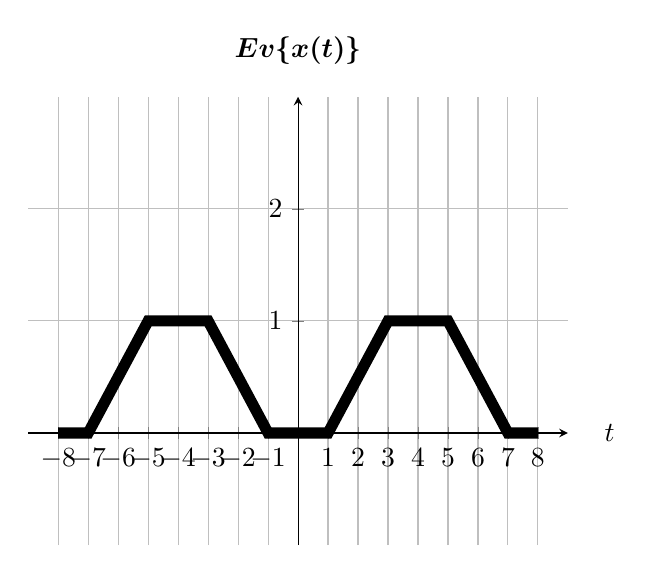
\begin{tikzpicture}[scale=1.0]
           \begin{axis}[
          axis lines=middle,
          xlabel={$t$},
          ylabel={$\boldsymbol{Ev\{x(t)\}}$},
          xtick={-8,...,0, 1, 2, 3, ..., 8},
          ytick={0, 1, 2},
          ymin=-1, ymax=3,
          xmin=-9, xmax=9,
          every axis x label/.style={at={(ticklabel* cs:1.05)}, anchor=west,},
          every axis y label/.style={at={(ticklabel* cs:1.05)}, anchor=south,},
          grid,
        ]
           \path[draw,line width=4pt] (-8,0) -- (-7,0) -- (-5,1) -- (-3,1) -- (-1,0) -- (0,0) -- (1,0) -- (3,1) -- (5,1) -- (7,0) -- (8,0);
           \end{axis}
        \end{tikzpicture}
        
        \label{fig:q2}
    \end{figure}
    
    Odd decomposition of x(t):\\
    
    \begin{figure}[h!]
    \centering
        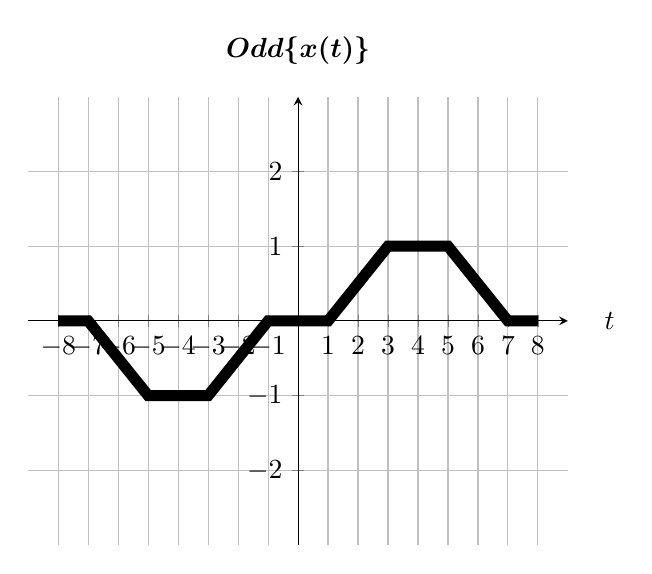
\begin{tikzpicture}[scale=1.0]
           \begin{axis}[
          axis lines=middle,
          xlabel={$t$},
          ylabel={$\boldsymbol{Odd\{x(t)\}}$},
          xtick={-8,...,0, 1, 2, 3, ..., 8},
          ytick={-2,-1,0, 1, 2},
          ymin=-3, ymax=3,
          xmin=-9, xmax=9,
          every axis x label/.style={at={(ticklabel* cs:1.05)}, anchor=west,},
          every axis y label/.style={at={(ticklabel* cs:1.05)}, anchor=south,},
          grid,
        ]
           \path[draw,line width=4pt] (-8,0) -- (-7,0) -- (-5,-1) -- (-3,-1) -- (-1,0) -- (0,0) -- (1,0) -- (3,1) -- (5,1) -- (7,0) -- (8,0);
           \end{axis}
        \end{tikzpicture}
        \label{fig:q2}
    \end{figure}
    
    \newpage

\item 
    \begin{enumerate}
    \item %write the solution of q6a
    
    $x(t)=u(t-1)-3u(t-3)+4u(t-4)$\\
    
    \item %write the solution of q6b
    \textbf{} \\
    \begin{center}
    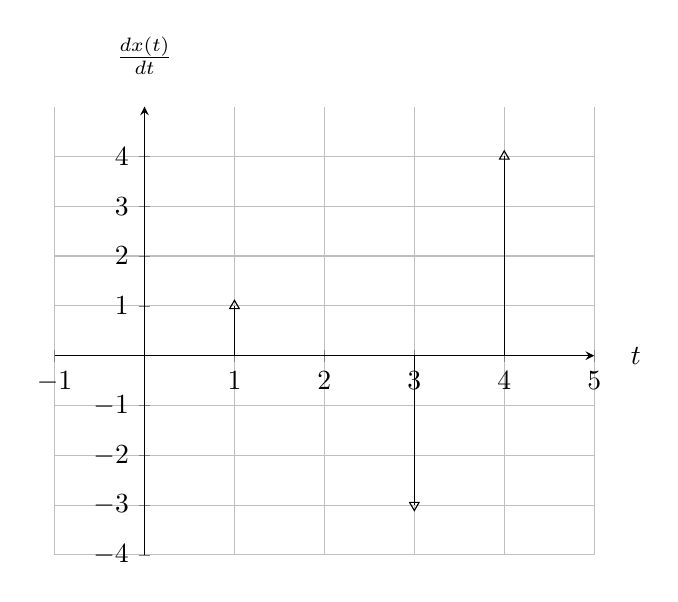
\begin{tikzpicture}
    \begin{axis}[ xlabel=$t$, ylabel=$\frac{dx(t)}{dt}$,
    xtick={},
    ytick={-4,-3,-2,-1,0,1,2,3,4},
    axis x line=center, axis y line = center, xmin=-1, xmax=5, ymin=-4, ymax=5,
    every axis x label/.style={at={(ticklabel* cs:1.05)}, anchor=west,},
          every axis y label/.style={at={(ticklabel* cs:1.05)}, anchor=south,},
          grid,]
    \addplot+[color=black,ycomb,mark=triangle,mark options={rotate=180}] plot coordinates {(3,-3)};
    \addplot+[color=black, ycomb,mark=triangle,mark options={rotate=0}] plot coordinates {(1,1) (4,4)};
    \end{axis}
    \end{tikzpicture}
    \end{center}
    
    \end{enumerate}

\end{enumerate}
\end{document}

